% Overview : capabilities.tex
% Explain what capability additions have resulted from benchmarking

\begin{frame}
  \frametitle{Core Capability : Demand Functions}
  Many simulators require the ability to define demand functions. 
  Multiple approaches exist, including specifying demand at each time
  step. 

  \vspace{0.2cm}

  In order to provide a universal tool for simulation developers, a 
  symbolic function toolbox was developed. We currently support:
  \begin{itemize}
    \item Linear Functions
    \item Exponential Functions
    \item Piecewise Functions (Combinations of those above)
  \end{itemize}
\end{frame}

\begin{frame}[ctb!]
  \frametitle{Core Capability : Demand Functions}
  \begin{figure}[htbp!]
    \begin{center}
      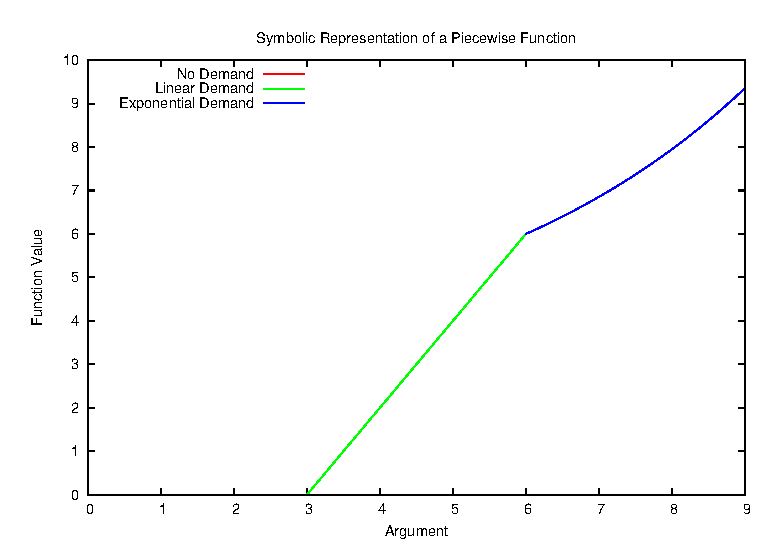
\includegraphics[height=5cm]{piecewise.eps}
    \caption{A piecewise function example using the Cyclus Symbolic 
      Function Toolbox}
    \label{fig:piecewisefunction}
    \end{center}
  \end{figure}
\end{frame}

\begin{frame}
  \frametitle{Core Capability : Facility Deployment}
  Cyclus now supports facility deployment in two modes, explicit 
  deployment and deployment in response to a defined demand.

  \vspace{1cm}

  Explicit deployment allows for user-defined deployment whereas 
  demand deployment allows for the process to be automated.

  \vspace{1cm}

  When more than one facility type meets a specific type of demand,
  an integer program (IP) is solved to determine the number and type of
  facilities to build.
\end{frame}

\begin{frame}
  \frametitle{Core Capability : Facility Deployment}
  In order to differentiate amongst facility types that meet a demand,
  a capacity and cost must be defined. At that point, the following IP
  is solved:

  %%% 
  \begin{subequations} \label{eqs:optBuild}
    \begin{equation} \label{eq:optBuildObj}
      \begin{aligned}
        & \min
        & & \sum_{f \in F}n_f*c_f
      \end{aligned}
    \end{equation}
    \begin{equation} \label{eq:optBuildConst}
      \begin{aligned}
        & \text{s.t.}
        & & \sum_{f \in F}n_f*\phi_f \ge \Phi
      \end{aligned}
    \end{equation}
    \begin{equation} \label{eq:optBuildBounds}
      \begin{aligned}
        & n_f \in [0,\infty) & \forall \:\: f \in F &
      \end{aligned}
    \end{equation}
    \begin{equation} \label{eq:optBuildInt}
      \begin{aligned}
        & n_f \:\: integer \:\: & \forall \:\: f \in F &
      \end{aligned}
    \end{equation}

    \vspace{0.2cm}
  
    where $\Phi$ is the unmet demand, $F$ is the set of facilities capable of 
    meeting the demand, and, for each facility in $F$, $c_f$ is the cost of building, 
    and $\phi_f$ is the nameplate capacity.  Finally, $n_f$ is the optimized number of
    facilities to build of type $f$.
  \end{subequations}
  %%% 
\end{frame}

\begin{frame}
  \frametitle{Core Capability : Enrichment and Resource Consumption}
  An Enrichment Toolbox has been added that provides methods to 
  calculate enrichment-related parameters. Calculable parameters 
  include:
  \begin{itemize}
    \item Uranium assay of a material
    \item Feed quantity required for enrichment
    \item Tails quantity resulting from enrichment
    \item SWU required for enrichment
  \end{itemize}
\end{frame}
